\documentclass[12pt,a4paper]{article}

% ── packages ───────────────────────────────────────────────────────────────
\usepackage[utf8]{inputenc}
\usepackage[T1]{fontenc}
\usepackage[english]{babel}
\usepackage{graphicx}
\usepackage{booktabs}
\usepackage{amsmath}
\usepackage{hyperref}
\usepackage{geometry}
\usepackage{caption}
\usepackage{float}

\geometry{margin=2.5cm}

\title{Custom-WikiCS Graph Exploration}
\author{}
\date{\today}

\begin{document}
\maketitle

% ═══════════════════════════════════════════════════════════════════════════
\section{Dataset Overview}
% ═══════════════════════════════════════════════════════════════════════════

The Custom-WikiCS graph is a directed graph derived from Wikipedia computer-science articles.
Each node represents an article, and each directed edge represents a hyperlink from one article to another.
In addition, every node is associated with a 1024-dimensional embedding vector produced by the
\textbf{BAAI/bge-m3} sentence-embedding model.  Because bge-m3 yields $\ell_2$-normalised vectors,
all pairwise Euclidean distances fall in the interval~$[0,2]$ and cosine similarity in~$[0,1]$.

\begin{itemize}
    \item \textbf{Nodes:} 11\,701
    \item \textbf{Edges:} 291\,039
    \item \textbf{Embedding dimension:} 1024
\end{itemize}

% ═══════════════════════════════════════════════════════════════════════════
\section{Degree Distribution}
% ═══════════════════════════════════════════════════════════════════════════

Figure~\ref{fig:degree_dist} shows the total, in-degree, and out-degree distributions.
All three are heavily right-skewed.  The total-degree histogram is dominated by a tall first
bin (degree~$<50$), with a long tail extending up to~3\,474.  The in-degree distribution is
even more extreme: over 10\,000 nodes have an in-degree below~50, and a handful of hub
articles attract over 3\,000 incoming links.
The out-degree histogram is comparatively compact (max~316) and shows a smoother decay;
its mean (24.87) falls near the beginning of the visible tail.

\begin{figure}[H]
    \centering
    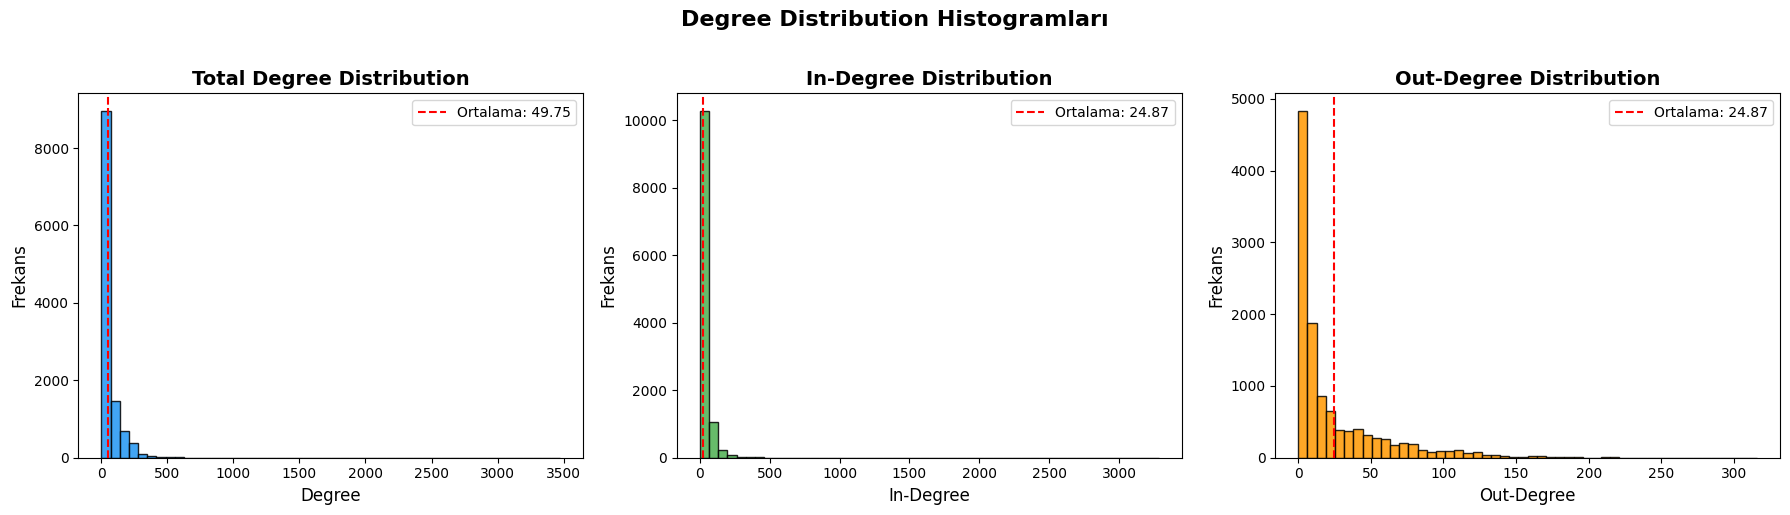
\includegraphics[width=\textwidth]{img-1-BAAI/degree_distribution.png}
    \caption{Degree distribution histograms (total, in-degree, out-degree).}
    \label{fig:degree_dist}
\end{figure}

\begin{table}[H]
\centering
\caption{Degree statistics.}
\label{tab:degree_stats}
\begin{tabular}{lrrrr}
\toprule
 & \textbf{Min} & \textbf{Max} & \textbf{Mean} & \textbf{Median} \\
\midrule
Total Degree  & 0 & 3\,474 & 49.75 & 14 \\
In-Degree     & 0 & 3\,283 & 24.87 & 4  \\
Out-Degree    & 0 & 316    & 24.87 & 9  \\
\bottomrule
\end{tabular}
\end{table}

\subsection{Log--Log Plot}

Figure~\ref{fig:degree_loglog} presents the degree distribution on log--log axes.
The points fall along an approximately straight line from degree~1 (frequency~$\sim$4\,000)
down to degree~$\sim$3\,500 (frequency~1), with mild convex curvature in the tail.
This nearly linear relationship on log--log axes is consistent with a power-law--like
distribution, which is a hallmark of scale-free networks.

\begin{figure}[H]
    \centering
    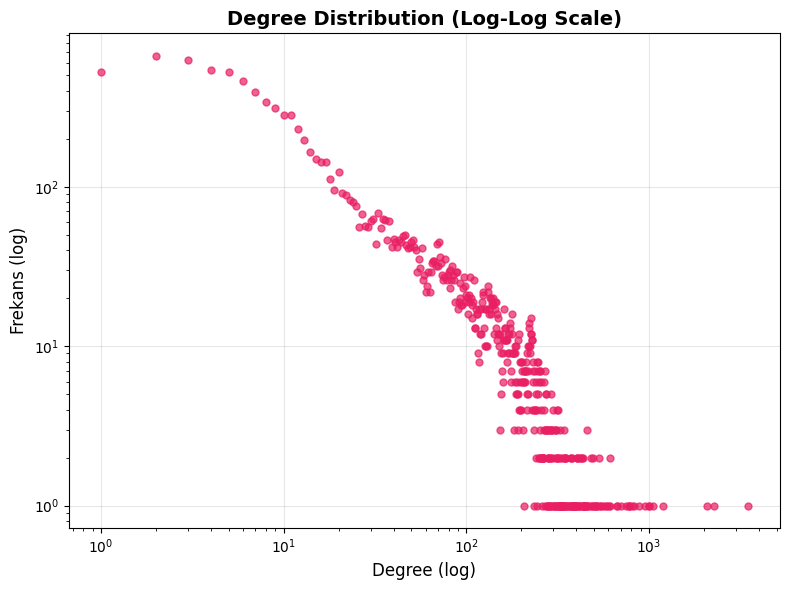
\includegraphics[width=0.65\textwidth]{img-1-BAAI/degree_distribution_loglog.png}
    \caption{Degree distribution on log--log scale.}
    \label{fig:degree_loglog}
\end{figure}

% ═══════════════════════════════════════════════════════════════════════════
\section{Degree Assortativity}
% ═══════════════════════════════════════════════════════════════════════════

The \emph{degree assortativity coefficient}~$r$ measures whether high-degree nodes
tend to connect to other high-degree nodes (\emph{assortative}, $r>0$) or to low-degree
nodes (\emph{disassortative}, $r<0$).

\[
    r = -0.0918
\]

The negative coefficient indicates that the graph is \textbf{disassortative}:
high-degree nodes tend to connect to low-degree nodes.
This is consistent with the typical structure of information networks (e.g., Wikipedia),
where a few highly-linked hub articles reference many less popular articles.

% ═══════════════════════════════════════════════════════════════════════════
\section{Topic--Link Structure Assortativity}
% ═══════════════════════════════════════════════════════════════════════════

To assess whether linked articles are also \emph{topically similar},
we compare the BAAI/bge-m3 embedding vectors of connected node pairs against those of
randomly sampled (unconnected) pairs using three metrics:
Cosine Similarity, Pearson Correlation, and Euclidean Distance.
Because the bge-m3 embeddings are $\ell_2$-normalised, cosine similarity and Pearson
correlation are expected to be nearly identical, and Euclidean distances are confined
to a narrow $[0,\sqrt{2}]$ range.

\subsection{Cosine Similarity}

\begin{figure}[H]
    \centering
    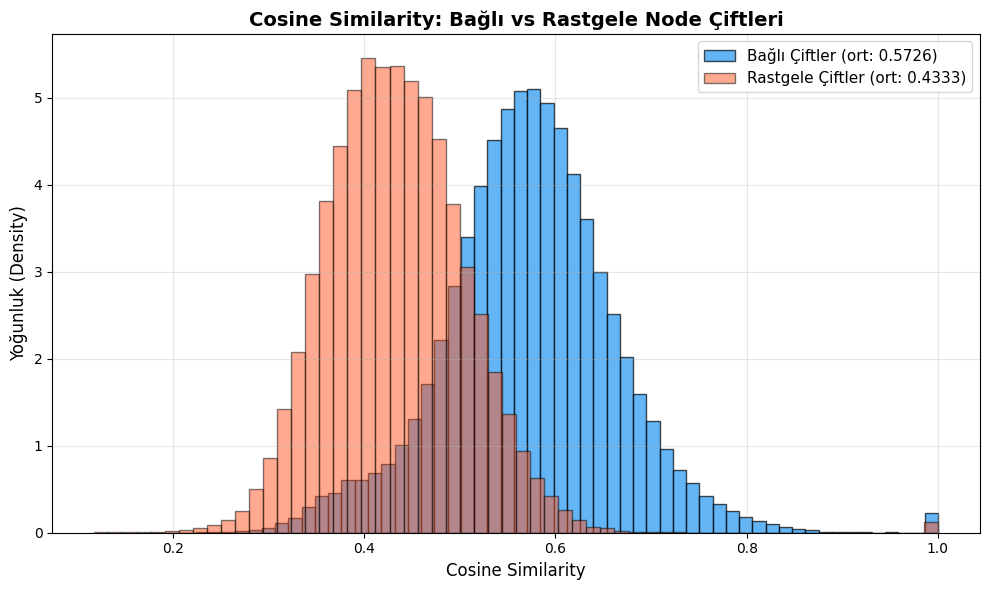
\includegraphics[width=0.8\textwidth]{img-1-BAAI/topic_link_cosine.png}
    \caption{Cosine similarity distribution: connected vs.\ random pairs.}
    \label{fig:cosine}
\end{figure}

\subsection{Pearson Correlation}

\begin{figure}[H]
    \centering
    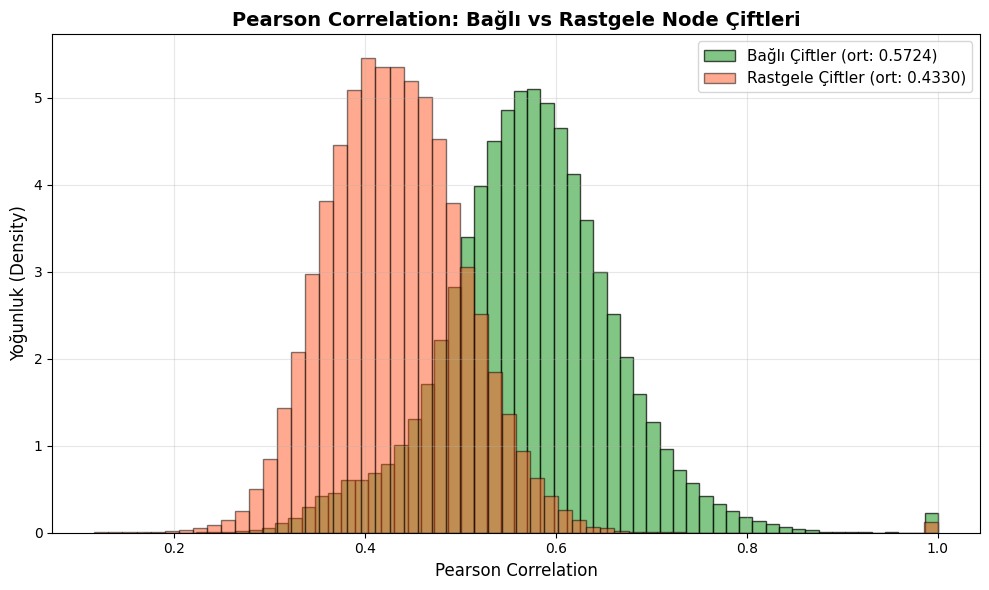
\includegraphics[width=0.8\textwidth]{img-1-BAAI/topic_link_pearson.png}
    \caption{Pearson correlation distribution: connected vs.\ random pairs.}
    \label{fig:pearson}
\end{figure}

\subsection{Euclidean Distance}

\begin{figure}[H]
    \centering
    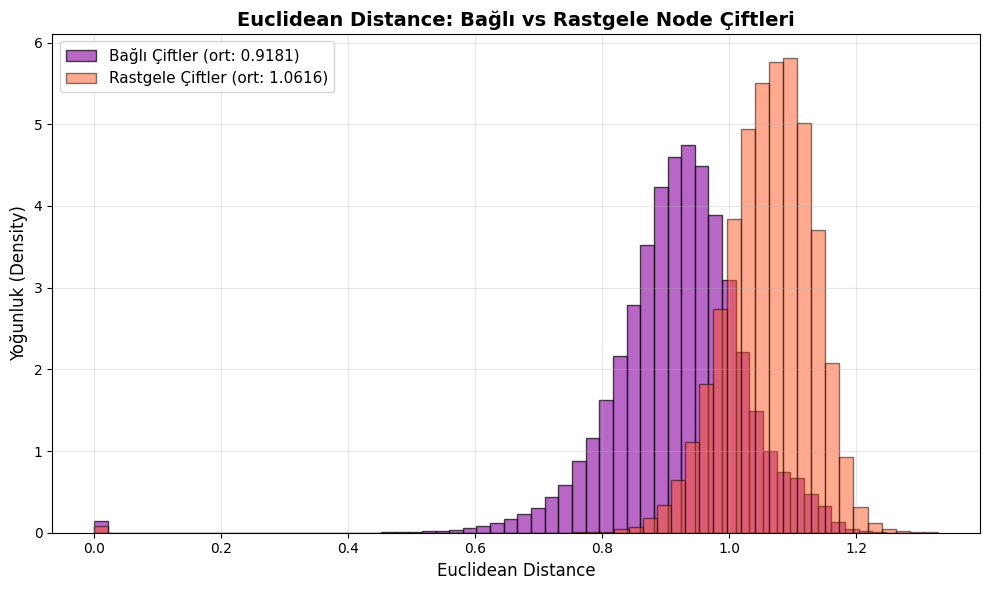
\includegraphics[width=0.8\textwidth]{img-1-BAAI/topic_link_euclidean.png}
    \caption{Euclidean distance distribution: connected vs.\ random pairs.}
    \label{fig:euclidean}
\end{figure}

\subsection{Summary}

Table~\ref{tab:topic_link} summarises the three metrics.
Connected pairs exhibit a cosine similarity of $0.5726$ on average, roughly $+0.14$
higher than the random baseline ($0.4333$).  Pearson correlation mirrors this almost
exactly ($0.5724$ vs.\ $0.4330$), as expected for normalised vectors.
For Euclidean distance, connected pairs are on average closer ($0.9181$) than random
pairs ($1.0616$), although the absolute gap~($-0.1435$) is small because the
normalised embedding space compresses all distances into $[0, \sim\!1.3]$.
The two distributions overlap substantially around~$0.9$--$1.1$, yet the shift is
statistically consistent: linked articles are indeed more topically similar than
arbitrary article pairs.  Notably, a small but visible spike near Euclidean
distance~$\approx 0$ reveals a set of near-duplicate or near-identical article pairs.

\begin{table}[H]
\centering
\caption{Topic--link assortativity summary.}
\label{tab:topic_link}
\begin{tabular}{lccccc}
\toprule
\textbf{Metric} & \textbf{Conn.\ Mean} & \textbf{Conn.\ Std} & \textbf{Rand.\ Mean} & \textbf{Rand.\ Std} & \textbf{Diff} \\
\midrule
Cosine Similarity   & 0.5726 & 0.0901 & 0.4333 & 0.0737 & +0.1393 \\
Pearson Correlation & 0.5724 & 0.0902 & 0.4330 & 0.0737 & +0.1394 \\
Euclidean Distance  & 0.9181 & 0.1089 & 1.0616 & 0.0802 & $-0.1435$ \\
\bottomrule
\end{tabular}
\end{table}

% ═══════════════════════════════════════════════════════════════════════════
\section{Local Transitivity (Clustering Coefficient)}
% ═══════════════════════════════════════════════════════════════════════════

The \emph{local clustering coefficient} of a node~$v$ measures how many of $v$'s
neighbours are also neighbours of each other.  High values indicate that $v$ sits
inside a tightly-knit cluster.

\begin{figure}[H]
    \centering
    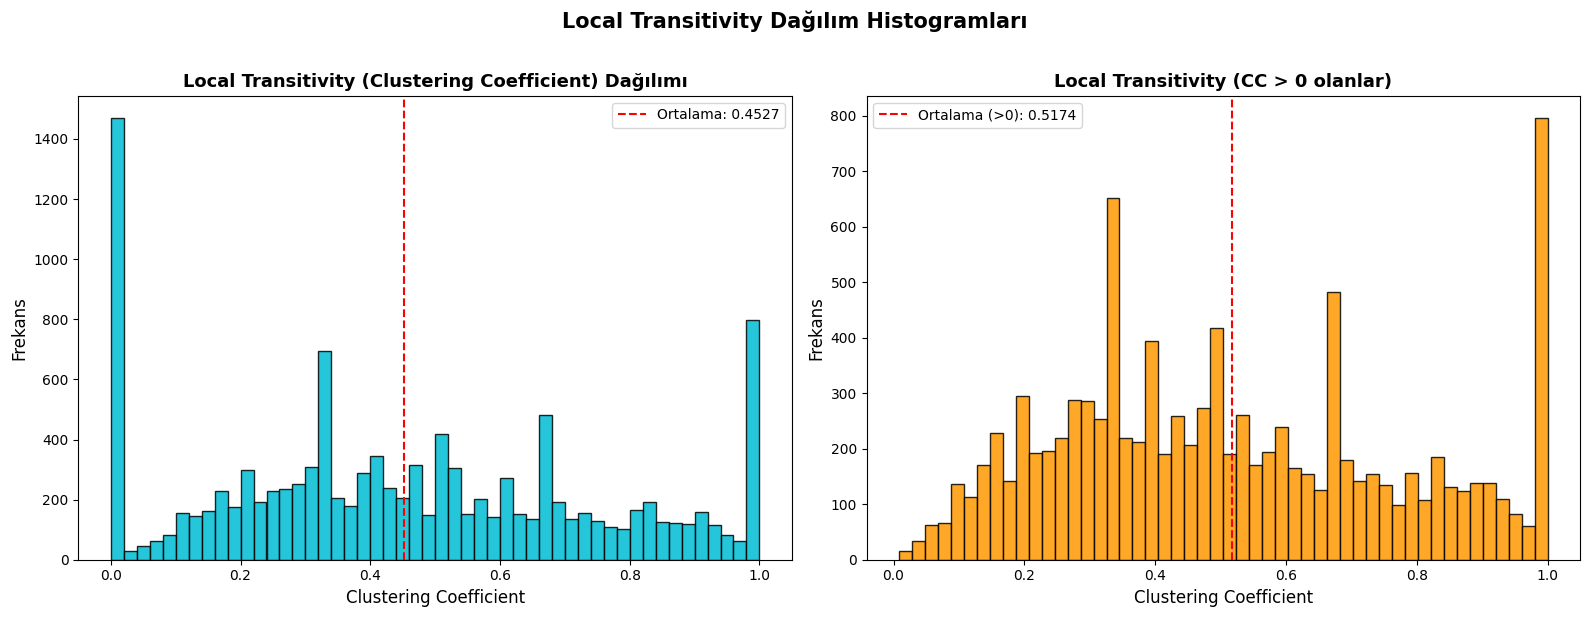
\includegraphics[width=\textwidth]{img-1-BAAI/local_transitivity.png}
    \caption{Local transitivity distribution: all nodes (left) and nodes with CC $> 0$ (right).}
    \label{fig:transitivity}
\end{figure}

\begin{table}[H]
\centering
\caption{Local transitivity statistics.}
\label{tab:cc_stats}
\begin{tabular}{lr}
\toprule
\textbf{Statistic} & \textbf{Value} \\
\midrule
Mean CC       & 0.4527 \\
Median CC     & 0.4286 \\
Min CC        & 0.0000 \\
Max CC        & 1.0000 \\
Std CC        & 0.2991 \\
Nodes with CC $= 0$ & 1\,463 \\
Nodes with CC $> 0$ & 10\,238 \\
Global Transitivity  & 0.2623 \\
\bottomrule
\end{tabular}
\end{table}

The left histogram shows a prominent spike at CC~$=0$ ($\sim$1\,460 nodes), followed
by a broad, roughly uniform spread across the $(0,1)$ interval with a secondary
concentration around CC~$\approx 0.33$ and a notable peak at CC~$=1.0$
($\sim$800 nodes with perfectly interconnected neighbourhoods).
When the zero-CC nodes are removed (right panel), the distribution shifts rightward
(mean~$=0.5174$), revealing a multimodal shape with peaks near $0.33$, $0.55$,
and~$1.0$.

The mean local clustering coefficient across all nodes is $0.4527$ with a global
transitivity of $0.2623$.  About $12.5\%$ of nodes have CC~$=0$; these are
either leaf nodes (degree~1) or nodes whose neighbours share no edges among
themselves.

% ═══════════════════════════════════════════════════════════════════════════
\section{Similarity Metrics vs.\ Node Degree}
% ═══════════════════════════════════════════════════════════════════════════

To investigate how topical similarity between linked articles relates to the
connectivity of the endpoints, Figure~\ref{fig:sim_degree} plots each of the
three similarity metrics (Cosine Similarity, Euclidean Distance, and Pearson
Correlation) against the degree of the source and target nodes of every edge.
All metrics use the BAAI/bge-m3 normalised embeddings, so the value ranges
are compact (cosine and Pearson in $[0.2,\,1.0]$; Euclidean in $[0,\,1.2]$).

\begin{figure}[H]
    \centering
    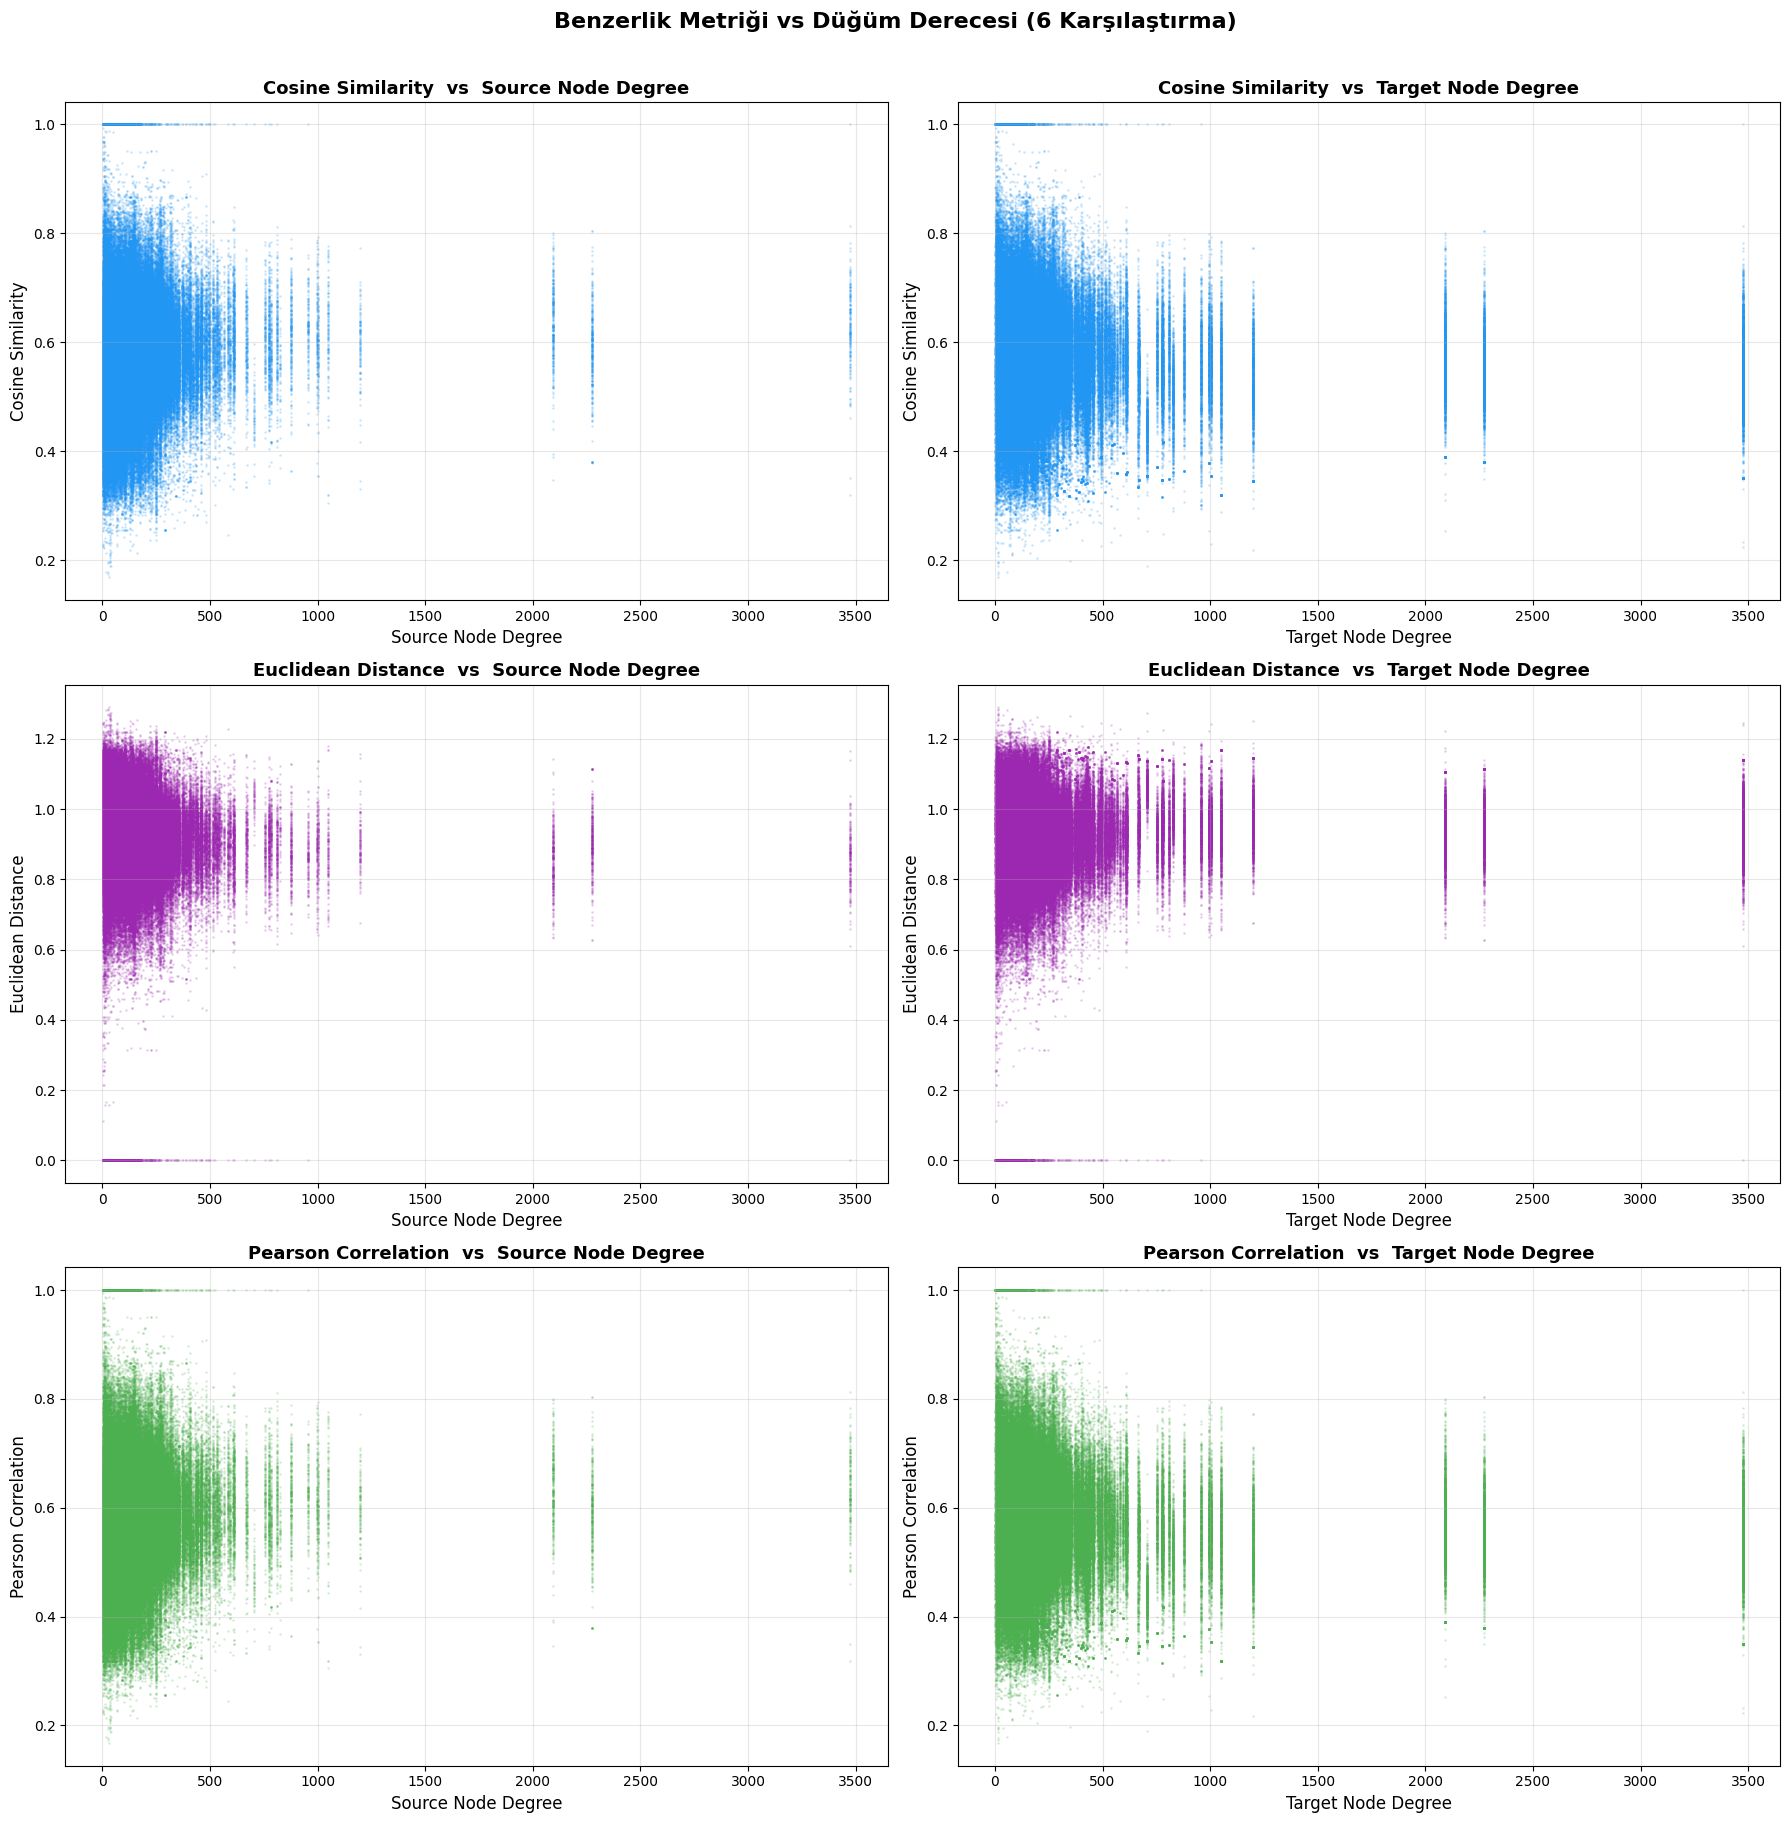
\includegraphics[width=\textwidth]{img-1-BAAI/similarityxdegree.png}
    \caption{Similarity metrics vs.\ node degree (source and target).
             Each row corresponds to a different metric; the left column uses
             the source node degree and the right column the target node degree.}
    \label{fig:sim_degree}
\end{figure}

Several observations emerge from the scatter plots:
\begin{itemize}
    \item For low-degree nodes (degree~$<500$) the similarity values
          span a wide range---cosine similarity stretches from $\sim$0.2
          to~1.0 and Euclidean distance from $\sim$0.0 to~1.2.
          As degree increases beyond $\sim$500, the spread narrows
          markedly and converges toward the global mean ($\sim$0.57 for
          cosine, $\sim$0.92 for Euclidean).  This variance reduction is
          expected: hubs connect to many diverse articles, so their
          per-edge similarity regresses toward the population average.
    \item A conspicuous horizontal band of points sits at Euclidean
          distance~$\approx 0$ (and cosine~$\approx 1.0$), especially
          prominent at low source and target degrees.  These correspond
          to near-duplicate or very closely related article pairs whose
          embeddings are almost identical.
    \item The Pearson correlation panels are virtually indistinguishable
          from the cosine panels, confirming that the bge-m3 embeddings
          are effectively $\ell_2$-normalised.
    \item The patterns are largely symmetric between source and target
          degree, consistent with the fact that topical similarity is an
          undirected property even though the graph itself is directed.
\end{itemize}

% ═══════════════════════════════════════════════════════════════════════════
\section{Cosine Similarity vs.\ Local Transitivity}
% ═══════════════════════════════════════════════════════════════════════════

Figure~\ref{fig:cos_cc} examines the relationship between the cosine
similarity of connected pairs and the local clustering coefficient (CC) of
the source and target nodes.

\begin{figure}[H]
    \centering
    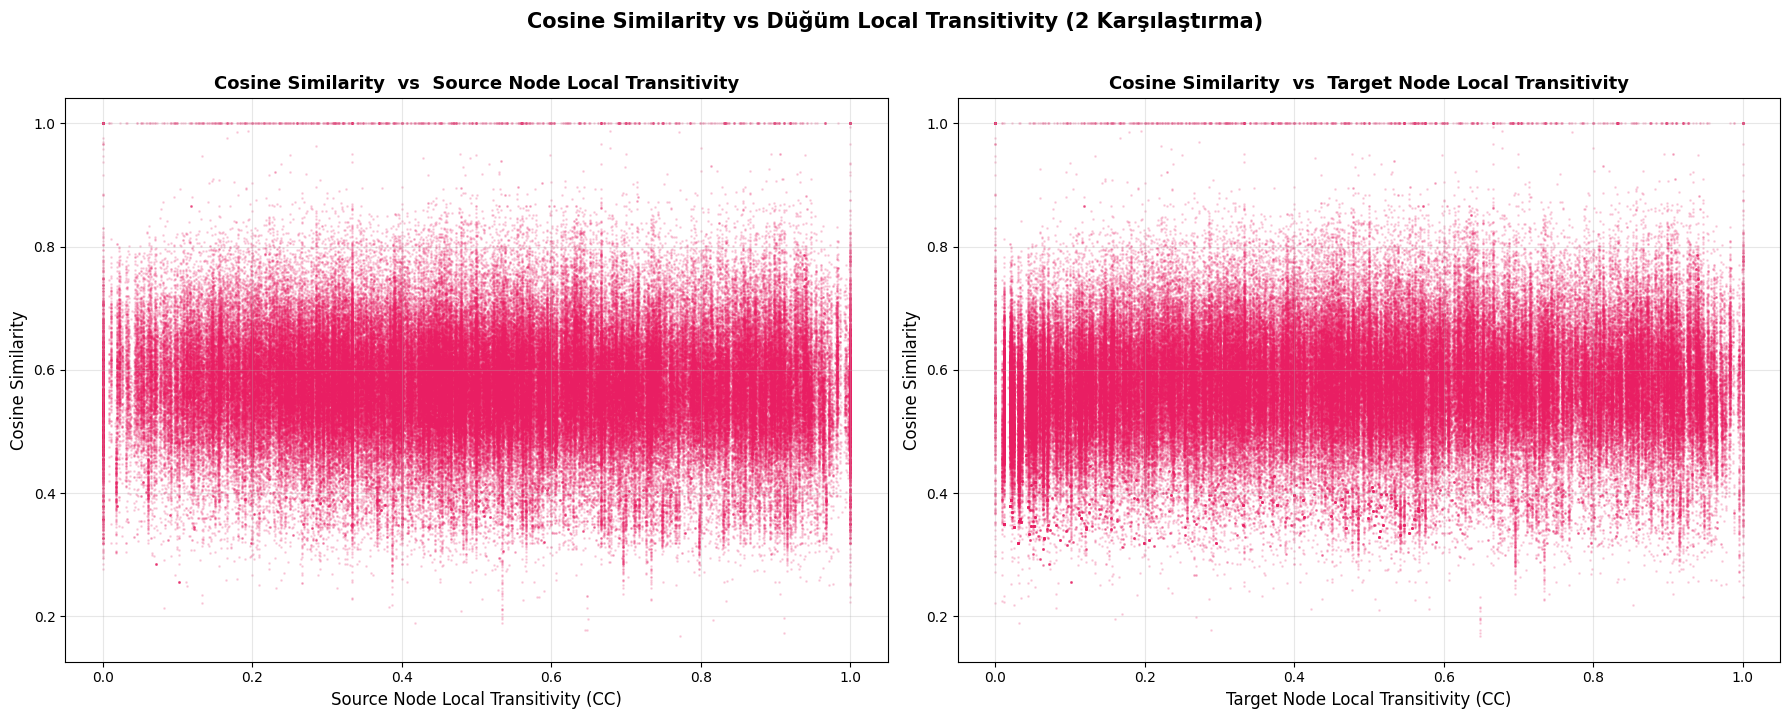
\includegraphics[width=\textwidth]{img-1-BAAI/cosinexlocaltransitivity.png}
    \caption{Cosine similarity vs.\ local transitivity of the source node
             (left) and the target node (right).}
    \label{fig:cos_cc}
\end{figure}

Both scatter plots display a dense, horizontally uniform cloud of points
with cosine similarity concentrated in the $0.4$--$0.7$ band.  Unlike some
other embedding models, there is \emph{no discernible positive or negative
trend} between local transitivity and cosine similarity: the cloud density
remains essentially flat from CC~$=0$ to CC~$=1$.
A thin but distinct horizontal line at cosine~$=1.0$ spans all CC values,
corresponding to near-duplicate article pairs.
The absence of a clear trend indicates that, under the BAAI/bge-m3
representation, local clustering structure is largely orthogonal to topical
similarity---a node can sit in a tightly-knit cluster of topically diverse
articles or in a sparse neighbourhood of topically similar ones.

\end{document}
